\documentclass[pdftex,12pt,a4paper]{article}

\usepackage{float}
\usepackage{graphicx}  
\usepackage[margin=2.5cm]{geometry}
\usepackage{breakcites}
\usepackage{indentfirst}
\usepackage{pgfgantt}
\usepackage{pdflscape}
\usepackage{float}
\usepackage{epsfig}
\usepackage{epstopdf}
\usepackage[cmex10]{amsmath}
\usepackage{stfloats}
\usepackage{multirow}
\setcounter{section}{-1}
\usepackage[%
    pdfborder={0 0 0}
]{hyperref}
\usepackage{listings}
\lstset{frame=tb,
  language=Java,
  aboveskip=3mm,
  belowskip=3mm,
  showstringspaces=false,
  columns=flexible,
  basicstyle={\small\ttfamily},
  numbers=none,
  breaklines=true,
  breakatwhitespace=true,
  tabsize=3
}


\renewcommand{\refname}{REFERENCES}
\linespread{1.3}

\usepackage{mathtools}
%\newcommand{\HRule}{\rule{\linewidth}{0.5mm}}
\thispagestyle{empty}
\begin{document}
\begin{titlepage}
\begin{center}
\textbf{}\\
\textbf{\Large{ISTANBUL TECHNICAL UNIVERSITY}}\\
\vspace{0.5cm}
\textbf{\Large{COMPUTER ENGINEERING DEPARTMENT}}\\
\vspace{2cm}
\textbf{\Large{BLG 222E\\ COMPUTER ORGANIZATION\\ PROJECT REPORT}}\\
\vspace{2.8cm}
\begin{table}[ht]
\centering
\Large{
\begin{tabular}{lcl}
\textbf{PROJECT NO}  & : & 1 \\
\textbf{GROUP NO}  & : & G71 \\
\end{tabular}}
\end{table}
\vspace{1cm}
\textbf{\Large{GROUP MEMBERS:}}\\
\begin{table}[ht]
\centering
\Large{
\begin{tabular}{rcl}
150220901  & : & MOHAMAD CHAHADEH \\
150190068  & : & ÖZGÜR SEFEROĞLU \\
150200913  & : & FITNETE GUNI
\end{tabular}}
\end{table}
\vspace{2.8cm}
\textbf{\Large{SPRING 2023}}

\end{center}

\end{titlepage}

\thispagestyle{empty}
\setcounter{tocdepth}{4}
\tableofcontents
\clearpage

\section{Introduction}

\subsection{Project Parts}
\begin{itemize}
\item Part 1: n-bit register
\item Part 2: Register Files \begin{itemize}
\item Part 2a: 16-bit IR Register
\item Part 2b: Register File (RF)
\item Part 2c: Address Register File (ARF)
\end{itemize}
\item Part 3: 8-bit ALU
\item Part 4: Whole System Integration
\end{itemize}

\subsection{Task Distribution}
\begin{enumerate}
\item ÖZGÜR SEFEROĞLU:  Part 3, Part 4
\item MOHAMAD CHAHADEH:  Part 1, Part 2a, Part 2b, Part 4
\item FITNETE GUNI: Part 2c, Part 4
\end{enumerate}

\pagebreak

\section{Part 1}
Implementing an n-bit Register, controlled using a 2-bit FunSel signal and an Enable signal. \hyperref[fig:part1_char]{Figure \ref{fig:part1_char}} Shows the diagram and characteristic equation of Part 1.

\begin{figure}[H]
\centering
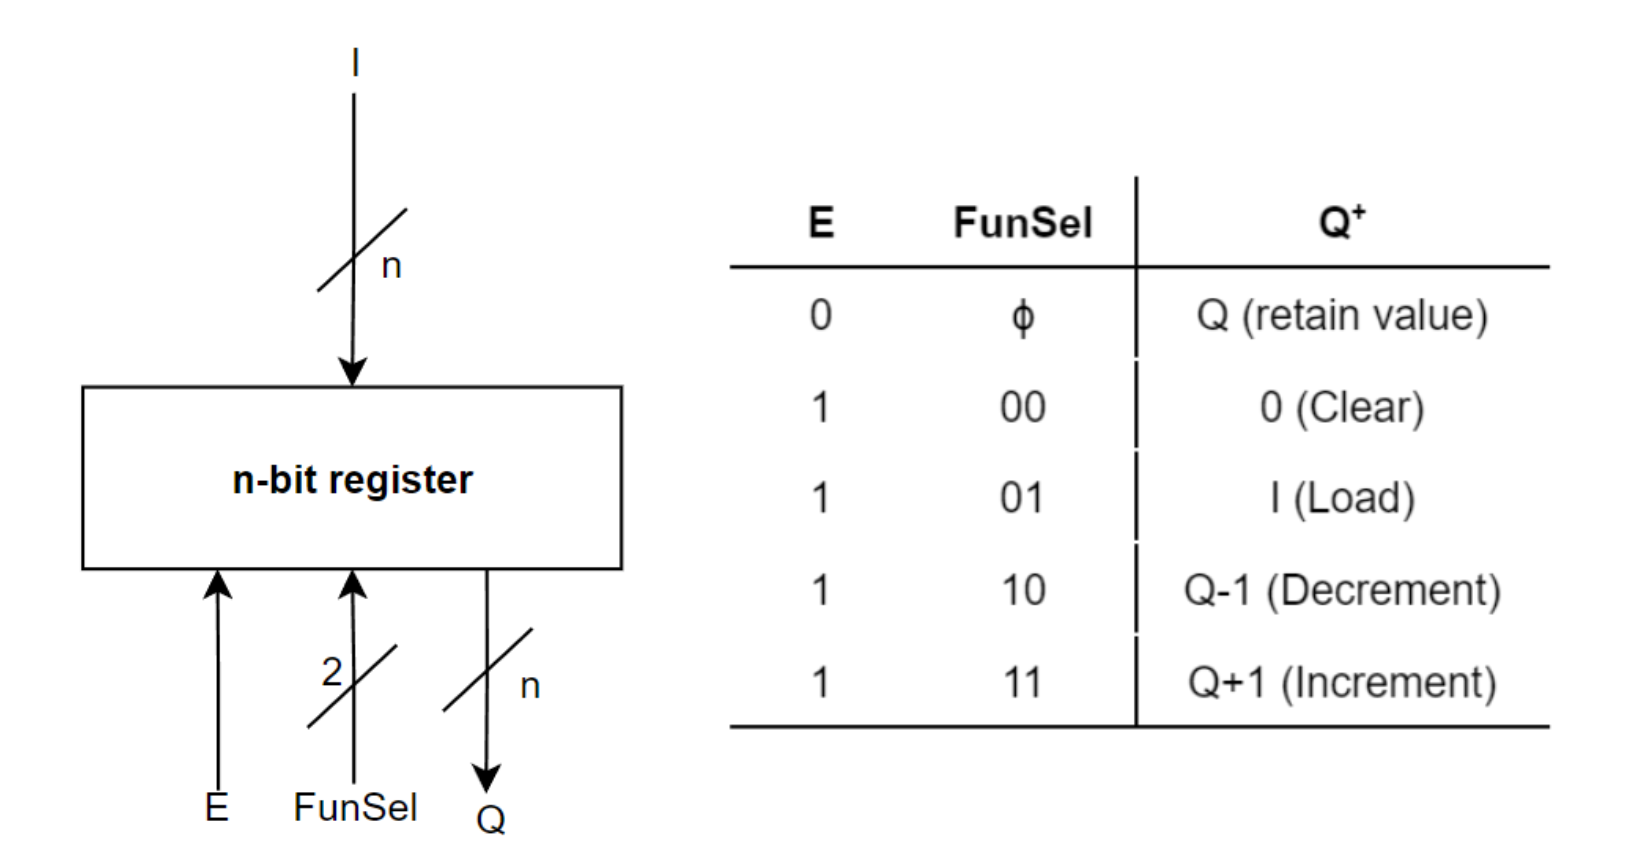
\includegraphics[width=0.7\textwidth]{part1_diagram.png}
\caption{Diagram and characteristic equation of Part 1}
\label{fig:part1_char}
\end{figure}

\subsection{Implementation}
the module implemented takes one parameter n, which is the number of bits of the register, a clock signal, two control inputs being FunSel and Enable, and one output of n-bits. the module is implemented by use the always block which executes on every positive edge of the clock, an if statement to check the enable signal, and a case block for the various inputs of FunSel. the following is the code for implementing the module.
\vspace{0.7cm}

\begin{lstlisting}
module part1 #(parameter n = 4) 
(input clk,
 input [1:0] FunSel,
 input [n-1:0] data_in, 
 input enable, 
 output reg [n-1:0] data_out);

    wire [n-1:0] zero = 0;
    always @(posedge clk)
    begin
        if (enable == 0)
            data_out <= data_out;
        else
            case (FunSel)
                2'b00: data_out <= zero;
                2'b01: data_out <= data_in;
                2'b10: data_out <= data_out - 1;
                2'b11: data_out <= data_out + 1;
            endcase
    end
endmodule
\end{lstlisting}

\subsection{Simulation}
\hyperref[fig:part1_sim]{Figure \ref{fig:part1_sim}} Shows a simulation of the module implemented earlier of n = 4.
\begin{figure}[H]
\centering
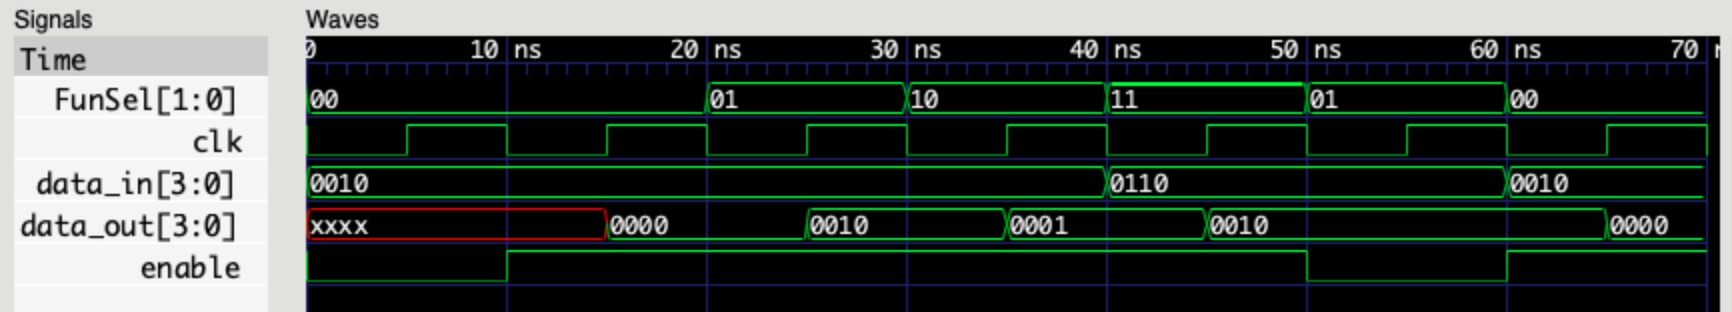
\includegraphics[width=1\textwidth]{part1_sim.png}
\caption{Simulation of Part 1, n-bit Register.}
\label{fig:part1_sim}
\end{figure}

\section{Part 2}

\subsection{Part 2a}
Designing a 16-bit IR Register whose Diagram and Characteristic table is shown in \hyperref[fig:part2a_diagram]{Figure \ref{fig:part2a_diagram}}.

\begin{figure}[H]
\centering
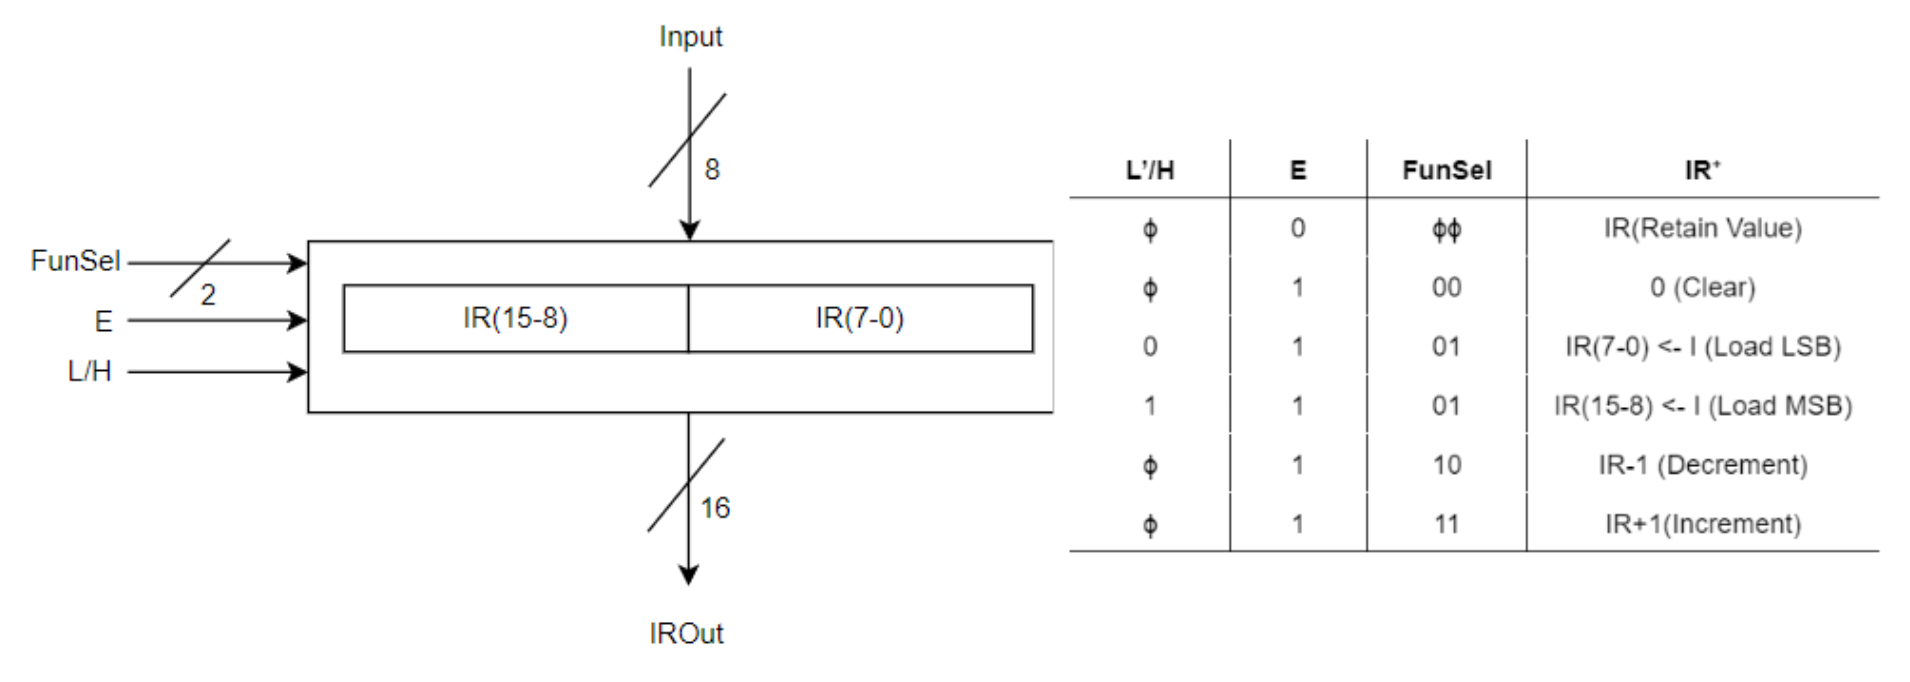
\includegraphics[width=0.7\textwidth]{part2a_diagram.png}
\caption{Diagram and Characteristics of Part 2a}
\label{fig:part2a_diagram}
\end{figure}

\end{document}